% !Mode:: "TeX:UTF-8"
%!TEX program  = xelatex

\documentclass[bwprint]{gmcmthesis}
\usepackage{CJK}
\usepackage{color}
\title{航站楼扩增评估}
\baominghao{4321} %参赛队号
\schoolname{武汉大学}%学校名称
\membera{戴非} %队员A
\memberb{周宇明} %队员B
\memberc{焦冲} %队员C
\begin{document}

 \maketitle

\begin{abstract}
我国航空运输业长期以来处于快速发展的状态,导致航空公司如今面临着一些挑战。其中登机口分配问题是日常生活中最重要的问题,不佳的分配方案会导致资源
浪费以及降低乘客乘坐的满意度,因此解决这个问题主要是为了保证乘客最大便利性的同时最小化所用登机口的数量。国内大量专家学者已对登机口优化问题进行
了研究也在此方面取得了一些研究成果,但在如何保证乘客便利性方面的研究还不够成熟。因此,本文在研究最小化所用登机口的数量的基础上,针对旅客的便捷性
(总体最短流程时间以及紧张度)进行详细分析。


问题1主要涉及\textcolor{red}{数学的最优化处理问题},对于题目所提供的信息,针对20号的数据进行变量定义与组合,建立航班信息与登机口数量之间非
线性数学模型。通过离散化的思想,结合深度优先搜索的算法得到最少使用登机口数量,使得耗费的成本最低。



\keywords{航站楼\quad  登机口\quad   乘客满意度\quad  动态规划模型}
\end{abstract}

\pagestyle{plain}

%目录 不推荐加
\tableofcontents

\section{问题重述}

\subsection{引言}

随着经济的发展,旅游成为了一种大部分现代人的一种生活娱乐方式,传统的交通方式已无法满足人们的需求。近年来乘机旅游已经成为了一种普遍的旅游方式,
这也使得以往的机场资源配置跟不上日益增大的交通需求,其中最为关键的是登机口的合理分配,原来的机场往往根据自身的经验进行登机口的分配和调度,
使得登机口航班组合没有达到最优,从而降低了登机口的利用效率。

\subsection{问题的提出}

\subsubsection{问题的提出内容一}

围绕创意平板折叠桌的动态变化过程、设计加工参数,本文依次提出如下问题:

(1)给定长方形平板尺寸 ($120 cm \times 50 cm \times 3 cm$),每根木条宽度(2.5 cm),连接桌腿木条的钢筋的位置,折叠后桌子的高度(53 cm)。要求建立模型描述此折叠桌的动态变化过程,并在此基础上给出此折叠桌的设计加工参数和桌脚边缘线的数学描述。



(2)折叠桌的设计应做到产品稳固性好、加工方便、用材最少。对于任意给定的折叠桌高度和圆形桌面直径的设计要求,讨论长方形平板材料和折叠桌的最优设计加工参数,例如,平板尺寸、钢筋位置、开槽长度等。对于桌高70 cm,桌面直径80 cm的情形,确定最优设计加工参数。


(3)给出软件设计的数学模型,可以根据客户任意设定的折叠桌高度、桌面边缘线的形状大小和桌脚边缘线的大致形状,给出所需平板材料的形状尺寸和切实可行的最优设计加工参数,使得生产的折叠桌尽可能接近客户所期望的形状,并根据所建立的模型给出几个设计的创意平板折叠桌。要求给出相应的设计加工参数,画出至少8张动态变化过程的示意图。

\section{模型的假设}
模型假设:
\begin{itemize}
\item 假设收集到的数据都具有真实性和代表新,可以作为各种计算的依据;
\item 假设航班能按时出发和达到;
\item 问题一只考虑航班—登机口分配;
\item 问题二不考虑乘客乘坐捷运和步行时间;
\item 假定临时机位数量无限定;
\end{itemize}

\section{符号说明}

\begin{tabular}{cc}
 \hline
 \makebox[0.4\textwidth][c]{符号}	&  \makebox[0.5\textwidth][c]{意义} \\ \hline
 P	    & 当前到达飞机  \\ \hline
 G	    & 当前可用登机口  \\ \hline
 PL	    & 当前停靠登机口飞机  \\ \hline
 GL	    & 当前空闲飞机  \\ \hline
 K      & K阶段 \\ \hline
 K+1    & K+1 \\ \hline
$S_{k}$   & 第K阶段状态 \\ \hline
$U_{k}$   & 第K阶段决策 \\ \hline
$U_{k+1}$ & 第K+1阶段状态 \\ \hline

\end{tabular}

\section{问题分析}
合理的利用登机口,不仅可以为乘客提供良好的乘机体验,还可以为航空公司节约了资源成本。传统的登机口的分配方式有很多不足,
所以如何建立起新的登机口分配方式引起了人们的广泛关注。\textcolor{red}{本文就这一问题建立了数学模型},分析了改良后的效果。
20号当天的航班图如下图1所示:
\begin{figure}[!h]
\centering
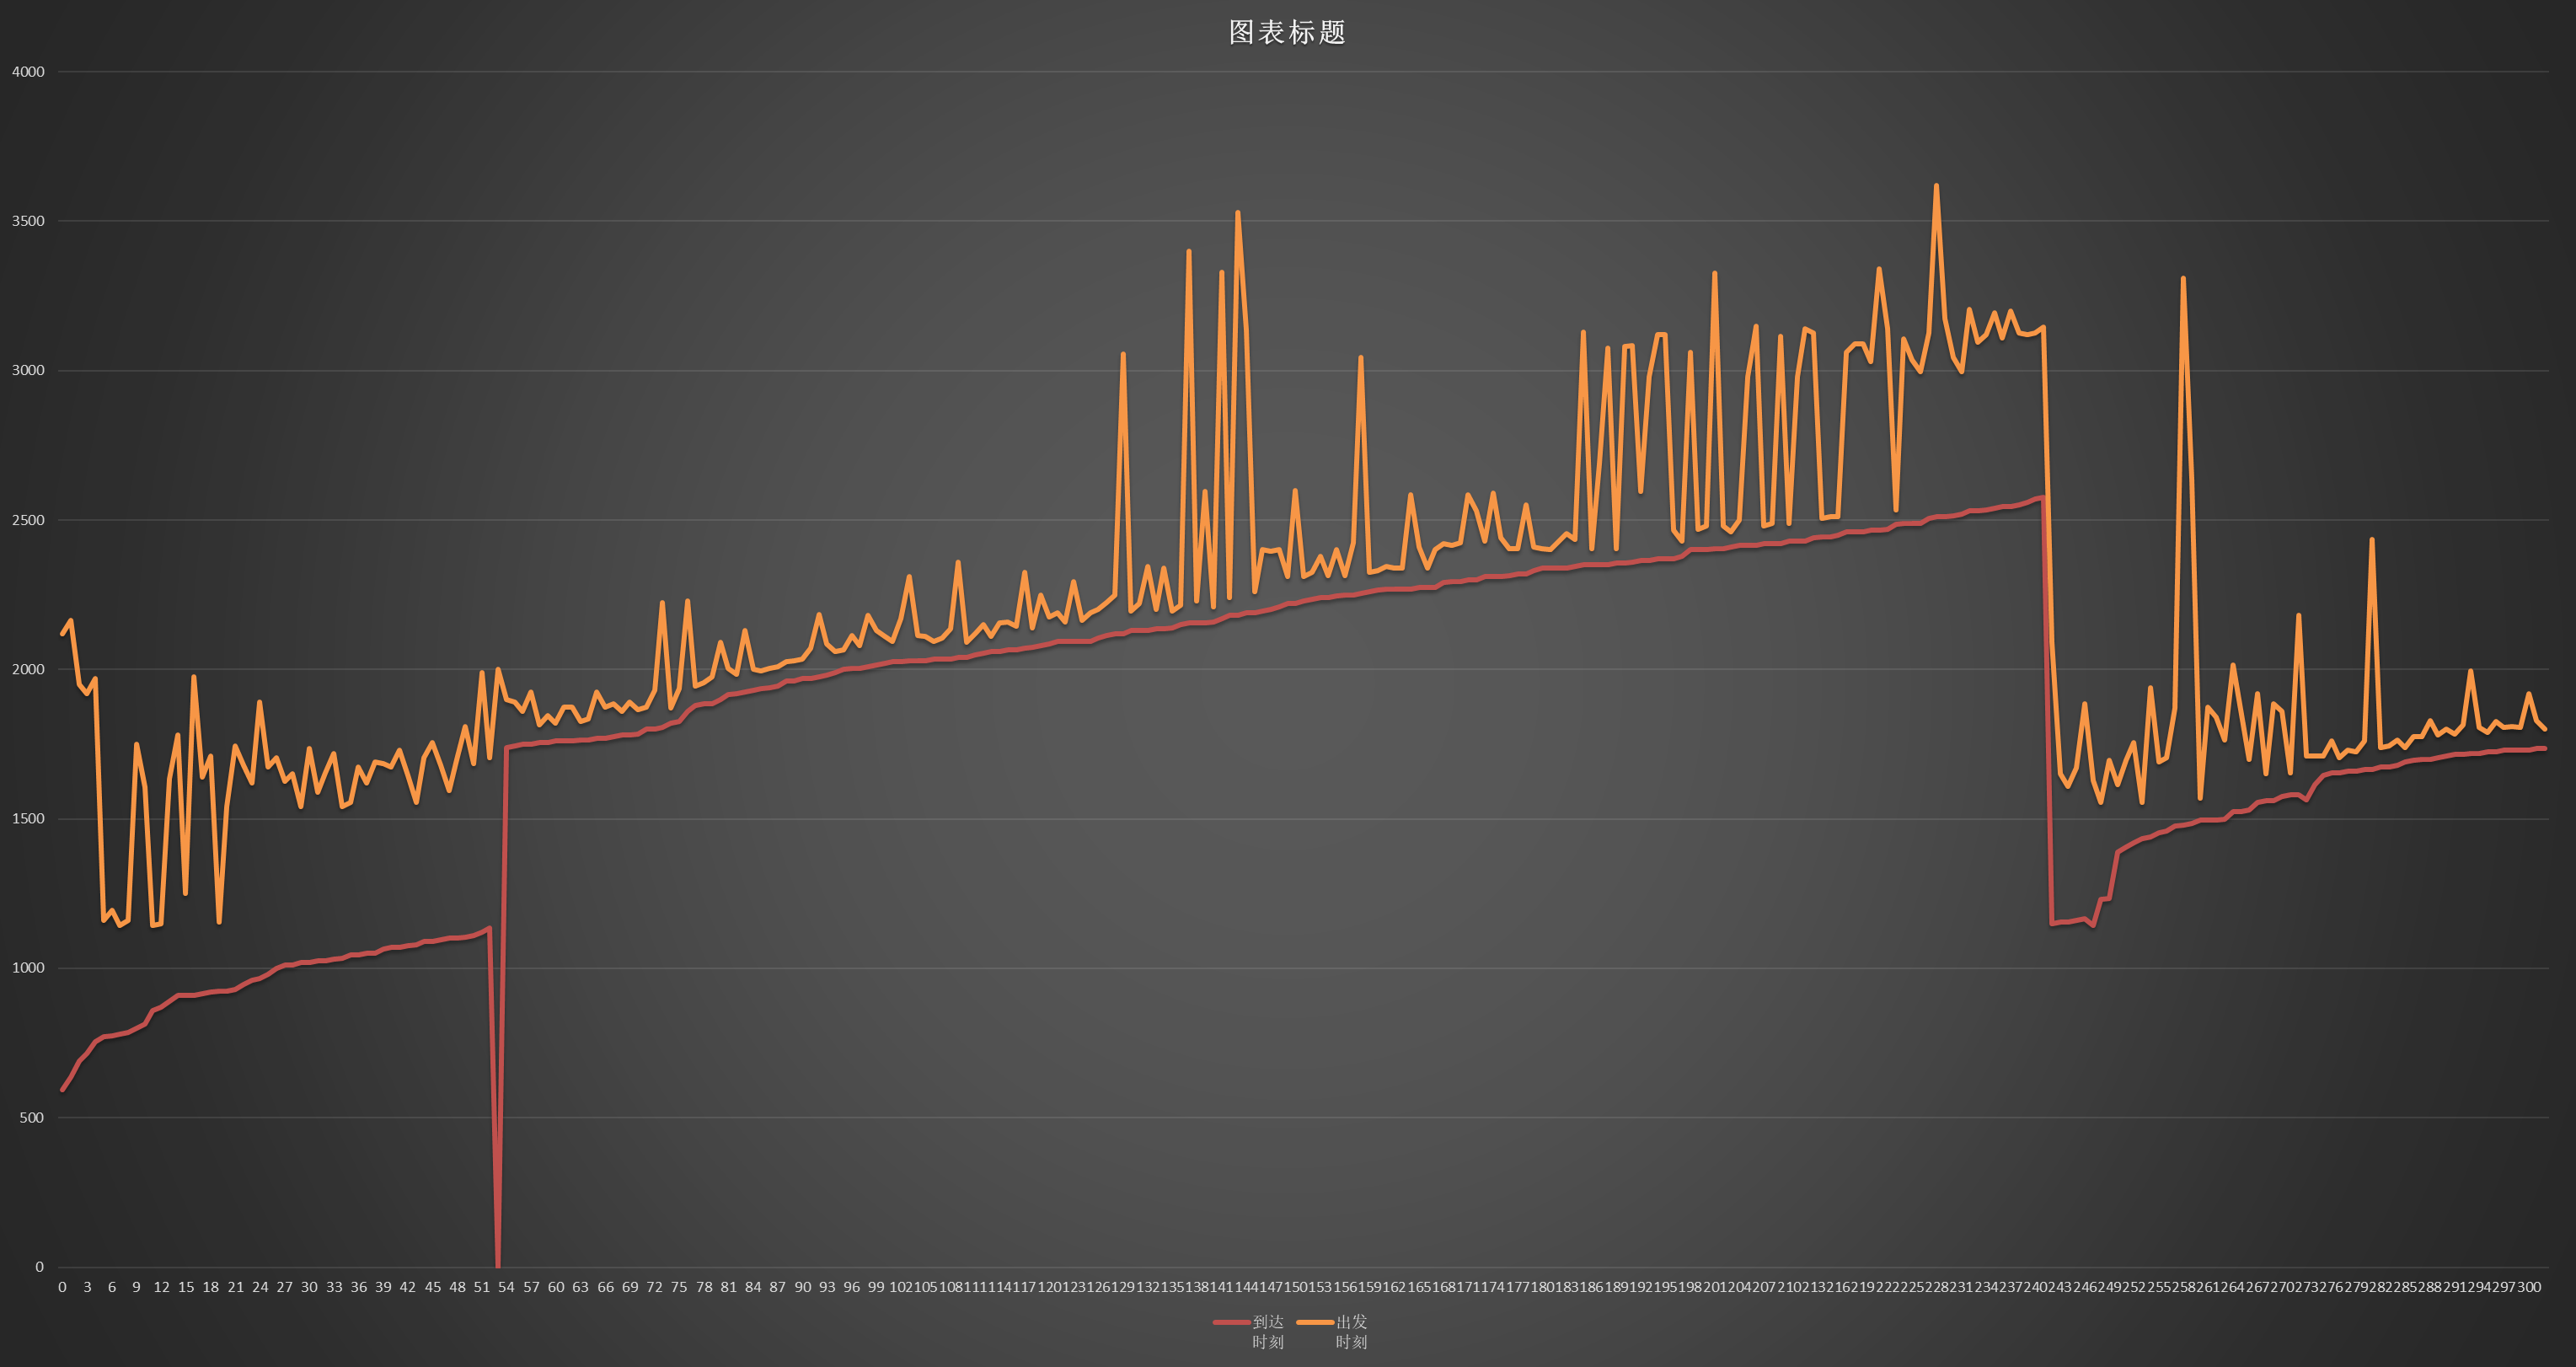
\includegraphics[width=.7\textwidth]{Figure1.png}
\caption{
横坐标代表航班的班次,纵坐标代表航班到达或起飞的时刻,初始时刻为20号最早航班时间。}
\end{figure}

\subsection{问题一分析}
问题1要求建立出能保证在尽可能多地分配航班到合适的登机口的同时,最小化登机口的数量。对于本文所提供的20号航班数据,某时刻
登机口的状态和最邻近45分钟之前的登机口的状态有关,故采用模型一的动态规划思想建立出动态转移方程,最后得到最小化登机口数量。
然后采用深度优先搜索得到的精确的结果进行模型的检验,发现能较好的保证结果的正确性。
\subsection{问题二分析}

\subsection{问题三分析}

\section{模型的建立与求解}

\subsection{最小化登机口数量模型}
\subsubsection{动态规划思想的运筹学模型}

%参考文献   手工录入
%\begin{thebibliography}{9}%宽度9
% \bibitem{bib:one} ....
% \bibitem{bib:two} ....
%\end{thebibliography}

%采用bibtex方案


\bibliographystyle{gmcm}
\bibliography{example}


\newpage
%附录
\appendix
%\setcounter{page}{1} %如果需要可以自行重置页码。
\section{我的 MATLAB 源程序}
\begin{lstlisting}[language=Matlab]%设置不同语言即可。
kk=2;[mdd,ndd]=size(dd);
while ~isempty(V)
[tmpd,j]=min(W(i,V));tmpj=V(j);
for k=2:ndd
[tmp1,jj]=min(dd(1,k)+W(dd(2,k),V));
tmp2=V(jj);tt(k-1,:)=[tmp1,tmp2,jj];
end
tmp=[tmpd,tmpj,j;tt];[tmp3,tmp4]=min(tmp(:,1));
if tmp3==tmpd, ss(1:2,kk)=[i;tmp(tmp4,2)];
else,tmp5=find(ss(:,tmp4)~=0);tmp6=length(tmp5);
if dd(2,tmp4)==ss(tmp6,tmp4)
ss(1:tmp6+1,kk)=[ss(tmp5,tmp4);tmp(tmp4,2)];
else, ss(1:3,kk)=[i;dd(2,tmp4);tmp(tmp4,2)];
end;end
dd=[dd,[tmp3;tmp(tmp4,2)]];V(tmp(tmp4,3))=[];
[mdd,ndd]=size(dd);kk=kk+1;
end; S=ss; D=dd(1,:);


 \end{lstlisting}


\end{document}
